
\chapter{Problems in one dimension}

To develop an understanding of finite elements further, we investigate several common one-dimensional problems.

%===============================================================================

\section{Second-order linear equation}

\index{Linear differential equations!1D}
  For the first example, we present the inner and outer singular-perturbation solution \index{Singular perturbation} \citep{logan_2006} to the second-order linear equation with non-constant coefficients, 
  \begin{align}
    \label{1d_example_1_ode}
    \epsilon \ddot{u} - (2t + 1)\dot{u} + 2u = 0, \hspace{5mm} 0 < t < 1, \hspace{5mm} 0 < \epsilon \ll 1,
  \end{align}
  \begin{align}
    \label{1d_example_1_bcs}
    u(0) = 1, \hspace{5mm} u(1) = 0,
  \end{align}
  and compare it to the solution obtained using the finite element method.

  \subsection{Singular perturbation solution}

  The solution to the unperturbed problem ($\epsilon = 0$) is found with the left boundary condition $u(0) = 1$:
  \begin{align*}
    - (2t + 1)\dot{u} + 2u = 0, \\
    \implies u(t) = c_1(2t + 1),
  \end{align*}
  applying the boundary condition $u(0) = 1$ results in the outer solution
  \begin{align*}
    u_o(t) = 2t + 1.
  \end{align*}
  In order to determine the width $\delta(\epsilon)$ of the \index{Boundary layer} boundary layer we re-scale near $t=1$ via
  \begin{align*}
    \xi = \frac{1 - t}{\delta(\epsilon)}, \hspace{10mm} U(\xi) = u(t).
  \end{align*}
  In scaled variables the differential equation becomes
  \begin{align*}
    \left( \frac{\epsilon}{\delta(\epsilon)^2} \right) \ddot{U} + \left( \frac{2 - 2\xi\delta(\epsilon) + 1}{\delta(\epsilon)}\right)\dot{U} + 2U &= 0 
  \end{align*}
  For this problem the second derivative term may be retained by making $\delta(\epsilon) = \bigo\left(\epsilon\right)$ resulting in the scaled differential equation
  \begin{align*}
    \left( \frac{\epsilon}{\epsilon^2} \right) \ddot{U} + \left( \frac{2 - 2\xi\epsilon + 1}{\epsilon}\right)\dot{U} + 2U &= 0 \\ 
    \ddot{U} + 3\dot{U} - 2\xi\epsilon \dot{U} + 2\epsilon U &= 0.
  \end{align*}
  The inner approximation to first-order satisfies
  \begin{align*}
    \ddot{U} + 3\dot{U} = 0,
  \end{align*}
  with general solution
  \begin{align*}
    U(\xi) = C_1 + C_2 e^{-3\xi},
  \end{align*}
  and also in terms of $u$ and $t$,
  \begin{align*}
    u(t) = C_1 + C_2 \exp\left( -3\left( \frac{1 - t}{\epsilon} \right) \right).
  \end{align*}
  Applying the boundary condition $u(1) = 0$ in the boundary layer gives $C_1 = -C_2$, and the inner approximation is
  \begin{align*}
    u_i(t) = C_2 \left( \exp\left( \frac{3t - 3}{\epsilon} \right) - 1 \right).
  \end{align*}

  To find $C_2$, an overlap domain of order $\sqrt{\epsilon}$ and an appropriate intermediate scaled variable
  $$\eta = \frac{1 - t}{\sqrt{\epsilon}}.$$
  are introduced.  Thus $t = 1 - \eta\sqrt{\epsilon}$ and the matching conditions becomes (with $\eta$ fixed)
  \begin{align*}
    \lim_{\epsilon \rightarrow 0^+} u_o\left(1 - \eta\sqrt{\epsilon}\right) = \lim_{\epsilon \rightarrow 0^+} u_i\left(1 - \eta\sqrt{\epsilon}\right),
  \end{align*}
  or
  \begin{align*}
    0 = &+ \lim_{\epsilon \rightarrow 0^+} \exp\left( 2(1 - \eta\sqrt{\epsilon}) + 1 \right) \\
        &- \lim_{\epsilon \rightarrow 0^+} C_2\left(\exp\left(\frac{3(1 - \eta\sqrt{\epsilon}) - 3}{\epsilon} \right) - 1 \right) \\
    0 = &+ \lim_{\epsilon \rightarrow 0^+} \exp\left( 3 - 2\eta\sqrt{\epsilon} \right) \\
        &- \lim_{\epsilon \rightarrow 0^+} C_2\left(\exp\left(\frac{- 3\eta\sqrt{\epsilon}}{\epsilon} \right) - 1 \right) \\
    0 = &\ 3 + C_2 \implies C_2 = -3.
  \end{align*}
  A uniform approximation $y_u(t)$ is found by adding the inner and outer approximations and subtracting the common limit in the overlap domain, which is $3$ in this case.  Consequently,
  \begin{align*}
    u_u(t) &= 2t + 1 - 3 \left( \exp\left( \frac{3t - 3}{\epsilon} \right) - 1 \right) - 3 \\
    &= 2t - 3 \exp\left( \frac{3t - 3}{\epsilon} \right) + 1.
  \end{align*}

  \subsection{Finite element solution} \label{ssn_intro_sing_perp_one}
  
  We arrive at the weak form by taking the inner product of Equation \cref{1d_example_1_ode} with the test function $\phi$, integrating over the domain of the problem $\Omega$ and integrating the second derivative term by parts,
  \begin{align*}
    0 = &\int_{\Omega} \left[ \epsilon \ddot{u} - (2t + 1)\dot{u} + 2u \right] \phi \d{\Omega} \\
    0 = &\epsilon \int_{\Omega} \totder[2]{u}{t} \phi \d{\Omega} - \int_{\Omega} (2t + 1) \totder{u}{t} \phi \d{\Omega} + 2\int_{\Omega} u \phi \d{\Omega} \\
    0 = &+\epsilon \int_{\Gamma} \left( \totder{u}{t} \phi \right) n \d{\Gamma} - \epsilon \int_{\Omega} \totder{u}{t} \totder{\phi}{t} \d{\Omega} \\
    &- \int_{\Omega} (2t + 1) \totder{u}{t} \phi \d{\Omega} + 2\int_{\Omega} u \phi \d{\Omega},
  \end{align*}
  where $n$ is the outward-pointing normal to the boundary $\Gamma$.  Because the boundary conditions are both Dirichlet, the integral over the boundary are all zero (see test space \cref{test_space}).  Therefore, the variational problem reads: find $u \in \trialspace$ such that 
  \begin{align*}
    0 = - \epsilon \int_{\Omega} \totder{u}{t} \totder{\phi}{t} \d{\Omega} - \int_{\Omega} (2t + 1) \totder{u}{t} \phi \d{\Omega} + 2\int_{\Omega} u \phi \d{\Omega}.
  \end{align*}
  for all $\phi \in \testspace$.
    
  A weak solution to this weak problem using linear Lagrange interpolation functions \cref{linear_lagrange_functions} is shown in \cref{1d_bvp_1_image}, and was generated from \cref{1d_bvp_1_code}.

\pythonexternal[label=1d_bvp_1_code, caption={FEniCS solution to BVP \cref{1d_example_1_ode,1d_example_1_bcs}.}]{scripts/fenics_intro/1D_BVP_1.py}
  
  \begin{figure}
    \centering
      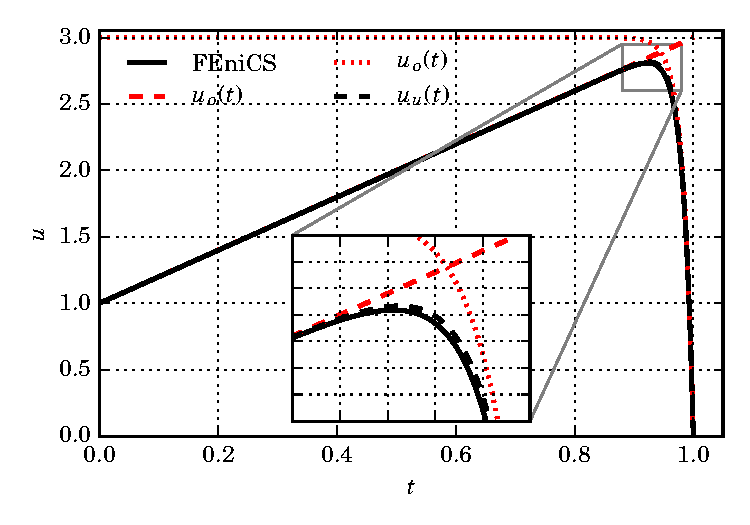
\includegraphics[width=\linewidth]{images/fenics_intro/1D_BVP_1.pdf}
    \caption[Singular-perturbation solution]{Finite element (solid black) and singular perturbation (dashed black) solutions.}
    \label{1d_bvp_1_image}
  \end{figure}

%===============================================================================

  \section{Neumann-Dirichlet problem}

\index{Linear differential equations!1D}
  It may also be of interest to solve a problem possessing a Neumann boundary condition.  For example, boundary conditions \cref{1d_example_1_bcs} for differential equation \cref{1d_example_1_ode} may be altered to 
  \begin{align}
    \label{1d_example_2_bcs}
    u(0) = 0, \hspace{10mm} \dot{u}(1) = u_r = -10.
  \end{align}
  In this case the weak form is derived similarly to \cref{ssn_intro_sing_perp_one}, and consists of finding $u \in \trialspace$ such that
  \begin{align*}
    0 = &+\epsilon \int_{\Gamma} \left( \totder{u}{t} \phi \right) n \d{\Gamma} - \epsilon \int_{\Omega} \totder{u}{t} \totder{\phi}{t} \d{\Omega} \\
    &- \int_{\Omega} (2t + 1) \totder{u}{t} \phi \d{\Omega} + 2\int_{\Omega} u \phi \d{\Omega} \\
    0 = &+\epsilon \int_{\Gamma_r} u_r \phi \d{\Gamma_r} - \epsilon \int_{\Omega} \totder{u}{t} \totder{\phi}{t} \d{\Omega} \\
    &- \int_{\Omega} (2t + 1) \totder{u}{t} \phi \d{\Omega} + 2\int_{\Omega} u \phi \d{\Omega},
  \end{align*}
  for all $\phi \in \testspace$, where the fact that $n = 1$ on the right boundary $\Gamma_r$.
    
    The weak solution using linear Lagrange shape functions \cref{linear_lagrange_functions} is shown in \cref{1d_bvp_2_image}, and was generated from \cref{1d_bvp_2_code}.

\pythonexternal[label=1d_bvp_2_code, caption={FEniCS solution to BVP \cref{1d_example_1_ode,1d_example_2_bcs}.}]{scripts/fenics_intro/1D_BVP_2.py}

  \begin{figure}
    \centering
      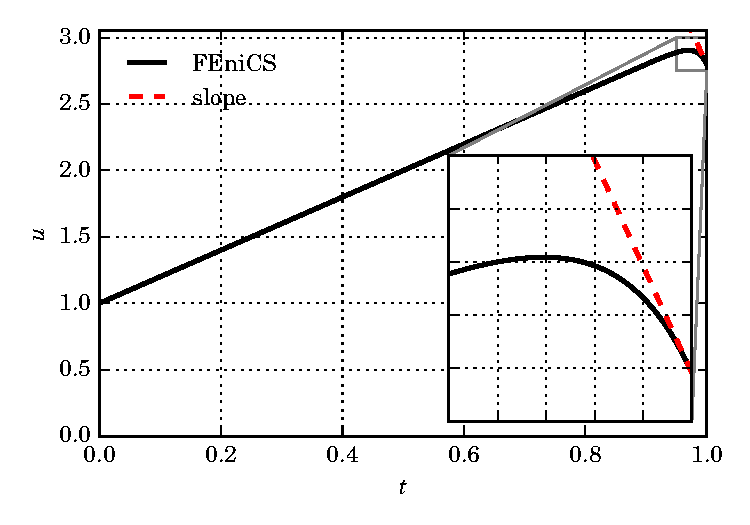
\includegraphics[width=\linewidth]{images/fenics_intro/1D_BVP_2.pdf}
    \caption[BVP example one solution]{Finite element solution (solid black) and slope (dashed red).}
    \label{1d_bvp_2_image}
  \end{figure}

%===============================================================================

  \section{Integration} \label{ssn_integration}
  
  \index{Numerical integration}
  An interesting problem easily solved with the finite element method is the integration of a function $u$ over domain $\Omega = [a,b]$,
  \begin{align}
    \label{numerical_integration_example}
    v(x) &= \int_a^x u(s) \d{s} = U(x) - U(a),
  \end{align}
  where $U$ is an anti-derivative of $u$ such that
  \begin{align*}
    \totder{U}{x} = u(x).
  \end{align*}
  Because the integral is from $a$ to $x$, $U(a) = 0$; hence $v(x) = U(x)$ and the equivalent problem to \cref{numerical_integration_example} is the first-order boundary-value problem
  \begin{align}
    \label{1d_example_4}
    \totder{v}{x} = u(x), \hspace{5mm} v(a) = 0.
  \end{align}

  The corresponding variational problem reads: find $v \in \trialspace$ such that
  \begin{align*}
    \int_{\Omega} \totder{v}{x} \phi \d{\Omega} &= \int_{\Omega} u \phi \d{\Omega},
  \end{align*}
  for all $\phi \in \testspace$.
  
  The linear-Lagrange-element-basis-weak solution to this problem with $u(x) = \cos(x)$ over the domain $\Omega = [0,2\pi]$ is shown in \cref{1d_bvp_4_image}, and was generated from \cref{1d_bvp_4_code}. 

\pythonexternal[label=1d_bvp_4_code, caption={FEniCS solution to BVP \cref{1d_example_4}}]{scripts/fenics_intro/1D_BVP_4.py}
  
  \begin{figure}
    \centering
      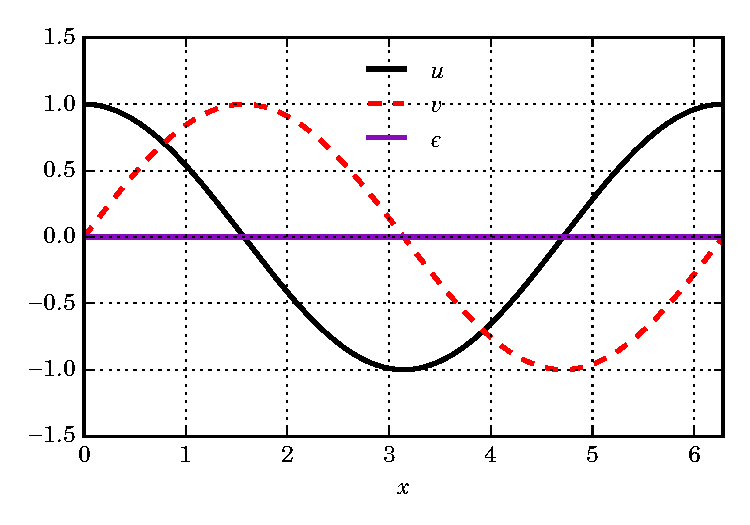
\includegraphics[width=\linewidth]{images/fenics_intro/1D_BVP_4.pdf}
    \caption[BVP example two solution]{The function $u(x) = \cos(x)$ for $a=0$, $b=2\pi$ (solid black); finite element solution $v(x) \approx \sin(x)$ (dashed red); and error $\epsilon(x) = v(x) - \sin(x)$ (purple solid).}
    \label{1d_bvp_4_image}
  \end{figure}

%===============================================================================
  
  \section{Directional derivative} \label{ssn_intro_directional_deriavative}
 
  \index{Directional derivative}
\index{Linear differential equations!1D}
  It is often important to compute the derivative of one function with respect to another, say
  \begin{align}
    \label{1d_example_5}
    w(x) = \totder{u}{v} = \totder{u}{x} \totder{x}{v} = \totder{u}{x} \left( \totder{v}{x} \right)^{-1},
  \end{align}
  for continuous functions $u(x)$ and $v(x)$ defined over the interval $\Omega = [a,b]$.  The variational form for this problem with trial function $w \in \ltwospace$ (see $L^2$ space \cref{l2_space}), test function $\phi \in \testspace$, is simply the inner product
   \begin{align*}
     \int_{\Omega} w \phi \d{\Omega} &= \int_{\Omega} \totder{u}{x} \left( \totder{v}{x} \right)^{-1} \phi \d{\Omega}, \hspace{5mm} \forall \phi \in \testspace,
   \end{align*}
   where no restrictions are made on the boundary; this is possible because both $u$ and $v$ are known \emph{a priori} and hence their derivatives may be computed directly and estimated throughout the entire domain.
   
   Solving problems of this type are referred to in the literature as \index{Projection} \emph{projections}, due to the fact that they simply project a known solution onto a finite element basis.
   
   An example solution with $u(x) = \sin(x)$, $v(x) = \cos(x)$ is generated using linear-Lagrange elements from \cref{1d_dir_dir_1_code} and depicted in \cref{1d_dir_dir_1_image},  and another with $u(x) = 3x^4$, $v(x) = x^6$ generated from \cref{1d_dir_dir_2_code} and depicted in \cref{1d_dir_dir_2_image}.

\pythonexternal[label=1d_dir_dir_1_code, caption={FEniCS solution to BVP \cref{1d_example_5} with $u(x) = \sin(x)$, $v(x) = \cos(x)$.}]{scripts/fenics_intro/1D_dir_dir_1.py}
  
  \begin{figure}
    \centering
      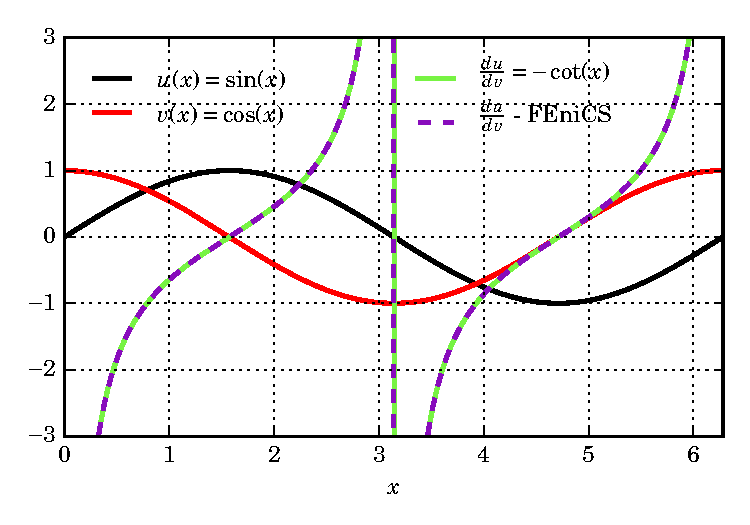
\includegraphics[width=\linewidth]{images/fenics_intro/1D_dir_dir_1.pdf}
    \caption[Functional derivative example one solution]{Both analytic (green) and numerical (purple) functional derivative $\totder{u}{v} = -\cot(x)$ for $u(x) = \sin(x)$ (black), and $v(x) = \cos(x)$ (red).}
    \label{1d_dir_dir_1_image}
  \end{figure}

\pythonexternal[label=1d_dir_dir_2_code, caption={FEniCS solution to BVP \cref{1d_example_5} with $u(x) = 3x^4$, $v(x) = x^6$.}]{scripts/fenics_intro/1D_dir_dir_2.py}
  
  \begin{figure}
    \centering
      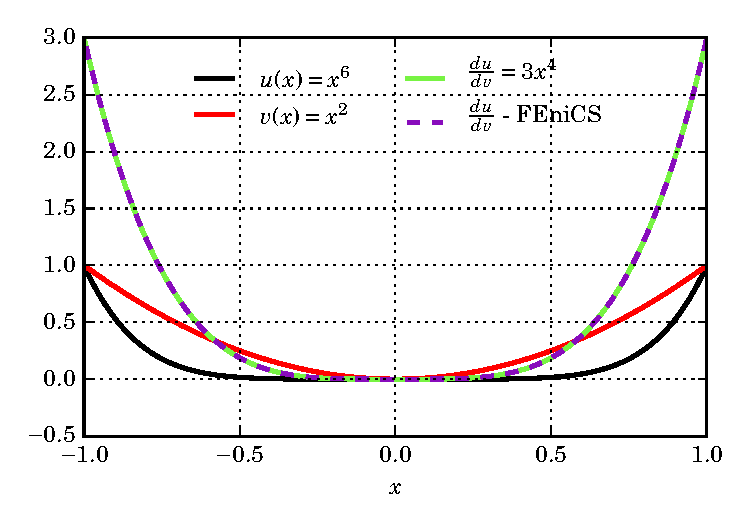
\includegraphics[width=\linewidth]{images/fenics_intro/1D_dir_dir_2.pdf}
    \caption[Functional derivative example two solution]{Both analytic (green) and numerical (purple) functional derivative $\totder{u}{v} = 3x^4$ for $u(x) = x^6$ (black), and $v(x) = x^2$ (red).}
    \label{1d_dir_dir_2_image}
  \end{figure}

%===============================================================================

\section{Eigenvalue problem}

\index{Transient problem}
\index{Eigenvalue problem}
The 1D initial-boundary-value problem for the heat equation with heat conductivity $k$ is
\begin{align}
  \label{intro_eigen_pde}
  \parder{u}{t} &= \parder{}{x} \left[ k \parder{u}{x} \right], &&0 < x < \ell,\ t > 0, \\
  \label{intro_eigen_bcs}
  u(0,t) &= u(\ell,t) = 0, &&t > 0, \\
  \label{intro_eigen_ic}
  u(x,0) &= f(x),       &&0 < x < \ell.
\end{align}
We examine this problem in the context of exact and approximate Eigenvalues and Eigenvectors in the following sections.

\subsection{Fourier series approximation}

\index{Fourier series method}
The solution of system \cref{intro_eigen_pde,intro_eigen_bcs,intro_eigen_ic} can be approximated by the method of separation of variables, developed by Joseph Fourier in 1822 \citep{davis_2013}.  Using this method, the partial derivative equation is transformed into a system of two ordinary differential equations.  First, assume a solution of the form $u(x,t) = X(x)T(t)$ so that equation \cref{intro_eigen_pde} reads
\begin{align*}
  X(x)\totder{T(t)}{t}  &= \totder{}{x} \left[ k \totder{X(x)}{x} \right] T(t) \\ 
  \frac{1}{k T(t)}\totder{T(t)}{t}  &= \frac{1}{X(x)} \totder{}{x} \left[ \totder{X(x)}{x} \right].
\end{align*}
For two functions with two different independent variables to be equal, they must both equal to the same constant $-\lambda$, $\lambda > 0$,
\begin{align*}
  \frac{1}{k T(t)}\totder{T(t)}{t} = \frac{1}{X(x)} \totder{}{x} \left[ \totder{X(x)}{x} \right] = - \lambda, 
\end{align*}
so
\begin{align}
  \label{intro_eigen_separated}
  \totder{T(t)}{t} + \lambda k T(t) = 0, \hspace{10mm} \totder[2]{X(x)}{x} + \lambda X(x) = 0.
\end{align}
The solution to the first-order $T$ equation is 
\begin{align}
  \label{intro_eigen_t}
  T(t) = Ae^{-\lambda k t},
\end{align}
while the solution to the second-order $X$ equation is
\begin{align*}
  X(x) = B_1 \sin\left( \sqrt{\lambda} x \right) + B_2 \cos\left( \sqrt{\lambda} x \right),
\end{align*}
for some coefficients $A$, $B_1$, and $B_2$ where $B_1$ and $B_2$ cannot both be zero since then only the trivial solution exists.  Applying boundary conditions \cref{intro_eigen_bcs}, $X(0) = X(\ell) = 0$,
\begin{align*}
  X(0) &= B_2 = 0, \\
  X(\ell) &= B_1 \sin\left( \sqrt{\lambda} \ell \right) = 0 &&\\
  \implies \sqrt{\lambda} \ell &= n\pi, &&n = 1,2,3,\dots \\
  \implies \lambda &= \left( \frac{n \pi}{\ell} \right)^2, &&n = 1,2,3,\dots
\end{align*}
Therefore, the Eigenfunctions and Eigenvalues for the steady-state problem are
\begin{align}
  \label{intro_eigen_x}
  X_n(x) = \sin\left( \sqrt{\lambda_n} x \right) \hspace{5mm}
  \lambda_n = \left( \frac{n \pi}{\ell} \right)^2, &&n = 1,2,3,\dots
\end{align}
By the Superposition Principle, any linear combination of solutions is again a solution, and solution to the transient problem is
\begin{align}
  u(x,t) &= \sum_{n=1}^{\infty} c_n X_n(x) T_n(t) \notag \\
  \label{intro_eigen_fourier_soln}
         &= \sum_{n=1}^{\infty} c_n \sin\left( \sqrt{\lambda_n} x \right) e^{-\lambda_n k t},
\end{align}
where $c_n = A B_1$ and \cref{intro_eigen_t} has been used with $\lambda_n = \left( \frac{n \pi}{\ell} \right)^2$.  The coefficient $c_n$ may be discovered by inspecting initial condition \cref{intro_eigen_ic}
\begin{align*}
  u(x,0) &= \sum_{n=1}^{\infty} c_n \sin\left( \sqrt{\lambda_n} x \right) = f(x).
\end{align*}
Multiplying both sides of this function by $\sin(m\pi x/\ell)$ for arbitrary $m$ and utilizing the fact that
\begin{align*}
  \int_{0}^{\ell} \sin\left(\frac{n\pi x}{\ell}\right) \sin\left(\frac{m\pi x}{\ell}\right) \d{x} \hspace{2mm} = \hspace{2mm}
  \begin{cases}
    0,      & n \neq m, \\
    \ell/2, & n = m,
  \end{cases}
\end{align*}
results in
{\footnotesize
\begin{align*}
  \sum_{n=1}^{\infty} c_n \sin\left( \frac{n\pi x}{\ell} \right) \sin\left(\frac{m\pi x}{\ell} \right) &= f(x) \sin\left( \frac{m\pi x}{\ell} \right) \\
  \int_{0}^{\ell} \sum_{n=1}^{\infty} c_n \sin\left( \frac{n\pi x}{\ell} \right) \sin\left(\frac{m\pi x}{\ell} \right) \d{x} &= \int_{0}^{\ell} f(x) \sin\left( \frac{m\pi x}{\ell} \right) \d{x} \\
  \sum_{n=1}^{\infty} c_n \int_{0}^{\ell} \sin\left( \frac{n\pi x}{\ell} \right) \sin\left(\frac{m\pi x}{\ell} \right) \d{x} &= \int_{0}^{\ell} f(x) \sin\left( \frac{m\pi x}{\ell} \right) \d{x} \\
  c_m \int_{0}^{\ell} \sin\left( \frac{m\pi x}{\ell} \right) \sin\left(\frac{m\pi x}{\ell} \right) \d{x} &= \int_{0}^{\ell} f(x) \sin\left( \frac{m\pi x}{\ell} \right) \d{x} \\
  c_m \left( \frac{\ell}{2} \right) &= \int_{0}^{\ell} f(x) \sin\left( \frac{m\pi x}{\ell} \right) \d{x}.
\end{align*}}
Finally, replacing the dummy variable $m$ with $n$,
\begin{align}
  \label{intro_eigen_fourier_coef}
  c_n = \frac{2}{\ell} \int_{0}^{\ell} f(x) \sin\left( \frac{n\pi x}{\ell} \right) \d{x}.
\end{align}

Therefore, the Fourier series approximation to \cref{intro_eigen_pde,intro_eigen_bcs,intro_eigen_ic} is \cref{intro_eigen_fourier_soln} with coefficients given by \cref{intro_eigen_fourier_coef}.

\subsection{Finite element approximation}

Investigating the Eigenvalue problem of separated equations \cref{intro_eigen_separated} for $X$,
\begin{align*}
  \totder[2]{X(x)}{x} + \lambda X(x) = 0, \hspace{5mm} X(0) = X(\ell) = 0,
\end{align*}
suggests that a weak form can be developed by making $X \in \trialspace$ and taking the inner product of this equation with the test function $\phi \in \testspace$
\begin{align}
  \int_0^{\ell} \left[ \totder[2]{X}{x} + \lambda X \right]\phi \d{x} &= 0 \notag \\
  \int_0^{\ell} \left[ \lambda X \phi - \totder{X}{x} \parder{\phi}{x} \right] \d{x} - \totder{X}{x} \phi(0) + \parder{X}{x} \phi(\ell) &= 0 \notag \\
  \label{intro_eigen_weak_form}
  \int_0^{\ell} \left[ \lambda X \phi - \totder{X}{x} \totder{\phi}{x} \right] \d{x} &= 0,
\end{align}
where the fact that the boundary conditions are all essential has been used.

Substituting the Galerkin approximation
\begin{align*}
  X_e = \sum_{j=1}^n u_j^e \psi_j^e(x),
\end{align*}
where $u_j^e$ is the $j$th nodal value of $X$ at element $e$ and $\psi_j^e(x)$ is the element's associated interpolation function, into Equation \cref{intro_eigen_weak_form} results in the Galerkin system
\begin{align*}
  \left[ \lambda M_{ij}^e - K_{ij}^e \right] \cdot \mathbf{u}^e = \mathbf{0},
\end{align*}
with stiffness tensor $K$ and \index{Mass matrix} \emph{mass tensor} $M$
\begin{align*}
  K_{ij}^e = \int_0^{\ell} \totder{\psi_i^e}{x} \totder{\psi_j^e}{x} \d{x}, \hspace{10mm} M_{ij}^e = \int_0^{\ell} \psi_i^e \psi_j^e \d{x}.
\end{align*}
Expanding the element equation tensors as in \cref{ssn_local_galerkin_assembly} results in
\begin{align*}
  \left( \frac{\lambda h_e}{6} \begin{bmatrix}[r]
                                 2 & 1 \\
                                 1 & 2
                               \end{bmatrix}
         - \frac{1}{h_e} \begin{bmatrix}[r]
                            1 & -1 \\
                           -1 & 1
                         \end{bmatrix}
  \right) \cdot
  \begin{bmatrix}
    u_1^e \\
    u_2^e\
  \end{bmatrix} &=
  \begin{bmatrix}
    0 \\
    0
  \end{bmatrix}.
\end{align*}

For a concrete example, we assemble this local system over an equally-space $n=3$-element function space, implying that $h_e = 1/3$ and (see \cref{ssn_global_galerkin_assembly})
{\footnotesize
\begin{align*}
  \left( \frac{\lambda}{18} \begin{bmatrix}[r]
                              2 & 1 & 0 & 0 \\
                              1 & 4 & 1 & 0 \\
                              0 & 1 & 4 & 1 \\
                              0 & 0 & 1 & 2 \\
                            \end{bmatrix}
         - 3 \begin{bmatrix}[r]
                1 & -1 &  0 &  0 \\
               -1 &  2 & -1 &  0 \\
                0 & -1 &  2 & -1 \\
                0 &  0 & -1 &  1
             \end{bmatrix}
  \right) \cdot
  \begin{bmatrix}
    X_1 \\
    X_2 \\
    X_3 \\
    X_4 \\
  \end{bmatrix} &=
  \begin{bmatrix}
    0 \\
    0 \\
    0 \\
    0
  \end{bmatrix}.
\end{align*}}
The boundary conditions $X(0) = X(\ell) = 0$ imply that $X_1 = X_4 = 0$ and thus this system reduces to a system of two linear equations,
\begin{align*}
  \left( \lambda \frac{4}{18} - 6 \right) X_2 + \left( \lambda\frac{1}{18} + 3 \right) X_3 &= 0 \\
  \left( \lambda \frac{1}{18} + 3 \right) X_2 + \left( \lambda\frac{4}{18} - 6 \right) X_3 &= 0,
\end{align*}
or
\begin{align*}
  \begin{bmatrix}
    \left( \lambda \frac{2}{9} - 6 \right) & \left( \lambda \frac{1}{18} + 3 \right) \\
    \left( \lambda \frac{1}{18} + 3 \right) & \left( \lambda \frac{2}{9} - 6 \right) \\
  \end{bmatrix} \cdot
  \begin{bmatrix}
    X_2 \\
    X_3 
  \end{bmatrix} &=
  \begin{bmatrix}
    0 \\
    0
  \end{bmatrix}.
\end{align*}
The characteristic polynomial is found by setting the determinant of the coefficient matrix equal to zero,
\begin{align*}
  \begin{vmatrix}
    \left( \lambda \frac{2}{9} - 6 \right) & \left( \lambda \frac{1}{18} + 3 \right) \\
    \left( \lambda \frac{1}{18} + 3 \right) & \left( \lambda \frac{2}{9} - 6 \right) \\
  \end{vmatrix} &= 0 \\
  \left( \lambda \frac{2}{9} - 6 \right) \left( \lambda \frac{2}{9} - 6 \right) - \left( \lambda \frac{1}{18} + 3 \right) \left( \lambda \frac{1}{18} + 3 \right) &= 0 \\
  \left( \lambda^2 \frac{4}{81} - \lambda \frac{24}{9} + 36 \right) - \left( \lambda^2 \frac{1}{324} + \lambda \frac{6}{18} + 9 \right) &= 0 \\
  \left( \frac{4}{81} - \frac{1}{324} \right) \lambda^2 - \left( \frac{24}{9} + \frac{6}{18} \right) \lambda + 27 &= 0 \\
  \left( \frac{5}{108} \right) \lambda^2 - 3 \lambda + 27 &= 0,
\end{align*}
with roots
\begin{align*}
  \lambda &= \frac{3 \pm \sqrt{9 - 108\left( \frac{5}{108} \right)}}{2\left( \frac{5}{108} \right)} = \frac{162}{5} \pm \frac{108}{5},
\end{align*}
providing the two Eigenvalue approximations $\widetilde{\lambda}_1 = 54/5 = 10.8$ and $\widetilde{\lambda}_2 = 54$.  The Eigenvectors may then be derived from the linear systems
\begin{align*}
  \begin{cases}
  \begin{bmatrix}
    \left( \widetilde{\lambda}_1 \frac{2}{9} - 6 \right) & \left( \widetilde{\lambda}_1 \frac{1}{18} + 3 \right) \\
    \left( \widetilde{\lambda}_1 \frac{1}{18} + 3 \right) & \left( \widetilde{\lambda}_1 \frac{2}{9} - 6 \right) \\
  \end{bmatrix} \cdot
  \begin{bmatrix}
    X_2^1 \\
    X_3^1 
  \end{bmatrix} &=
  \begin{bmatrix}
    0 \\
    0
  \end{bmatrix} \\
  \begin{bmatrix}
    \left( \widetilde{\lambda}_2 \frac{2}{9} - 6 \right) & \left( \widetilde{\lambda}_2 \frac{1}{18} + 3 \right) \\
    \left( \widetilde{\lambda}_2 \frac{1}{18} + 3 \right) & \left( \widetilde{\lambda}_2 \frac{2}{9} - 6 \right) \\
  \end{bmatrix} \cdot
  \begin{bmatrix}
    X_2^2 \\
    X_3^2 
  \end{bmatrix} &=
  \begin{bmatrix}
    0 \\
    0
  \end{bmatrix}
  \end{cases}&\\
  \begin{cases}
  \begin{bmatrix}
    -\frac{18}{5} &  \frac{18}{5} \\
     \frac{18}{5} & -\frac{18}{5} \\
  \end{bmatrix} \cdot
  \begin{bmatrix}
    X_2^1 \\
    X_3^1 
  \end{bmatrix} &=
  \begin{bmatrix}
    0 \\
    0
  \end{bmatrix} \\
  \begin{bmatrix}
    6 & 6 \\
    6 & 6 \\
  \end{bmatrix} \cdot
  \begin{bmatrix}
    X_2^2 \\
    X_3^2 
  \end{bmatrix} &=
  \begin{bmatrix}
    0 \\
    0
  \end{bmatrix}
  \end{cases}&
\end{align*}
providing $X^1 = \begin{bmatrix} 1 & 1 \end{bmatrix}\T$ and $X^2 = \begin{bmatrix} 1 & -1 \end{bmatrix}\T$.

Similar to the derivation of Fourier series solution \cref{intro_eigen_fourier_soln}, these approximate Eigenvectors and Eigenvalues are used to create the approximate three-element transient solution
\begin{align}
  u(x,t) \approx \widetilde{u}(x,t) &= \sum_{e=1}^n X^e(x) T^e(t, \widetilde{\lambda}_e) \notag \\
  \label{intro_eigen_fem_soln}
  &= \sum_{e=1}^3 \left[ \sum_{j=1}^2 X^e_j \psi_j^e(x) \right] c_e e^{-\widetilde{\lambda}_e k t},
\end{align}
where $c_e = c_n$ are the same coefficients of orthogonality as \cref{intro_eigen_fourier_coef} from the Fourier series approximation at element $e = n$, $n=1,2,3$, and $X^e$ is the Eigenvector associated with Eigenvalue $\widetilde{\lambda}_e$.

Results derived using initial condition $f(x) = 1$ in \cref{intro_eigen_ic} for an eight-term Fourier series approximation \cref{intro_eigen_fourier_soln,intro_eigen_fourier_coef} and an 8-element finite element approximation analogous to \cref{intro_eigen_fem_soln,intro_eigen_fourier_coef} are generated with \cref{eigenvalue_code}.
The resulting Eigenfunctions are plotted in \cref{1d_example_eigenvectors} and resulting approximations in \cref{1d_example_eigensolution}.

\pythonexternal[label=eigenvalue_code, caption={FEniCS code for solution of the Eigenvalue problem.}]{scripts/fenics_intro/eigenvalues.py}

\begin{figure*}
  \centering
    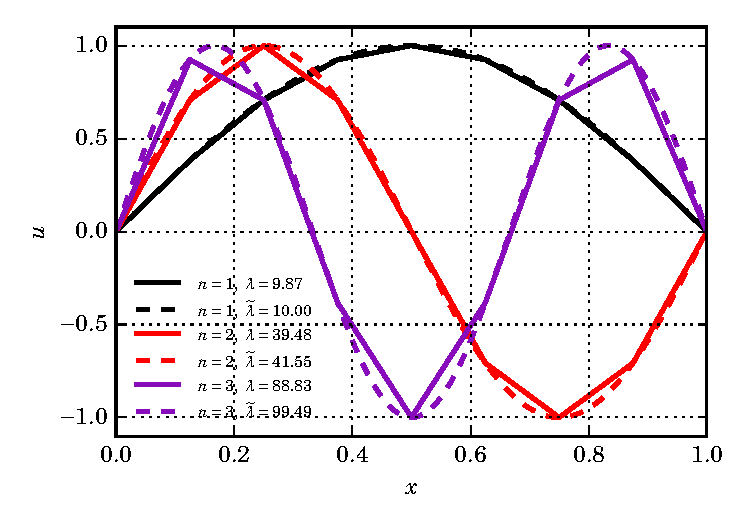
\includegraphics[width=0.7\linewidth]{images/fenics_intro/eigenvectors.pdf}
  \caption[Eigenvector example solution]{Fourier series Eigenfunctions (dashed) and 8 linear element finite element Eigenvectors (solid) for $n=1,2,3$.  The associated exact Eigenvalue $\lambda$ and FEM-approximated Eigenvalues $\tilde{\lambda}$ are listed in the legend.}
  \label{1d_example_eigenvectors}
\end{figure*}

\begin{figure*}
  \centering
    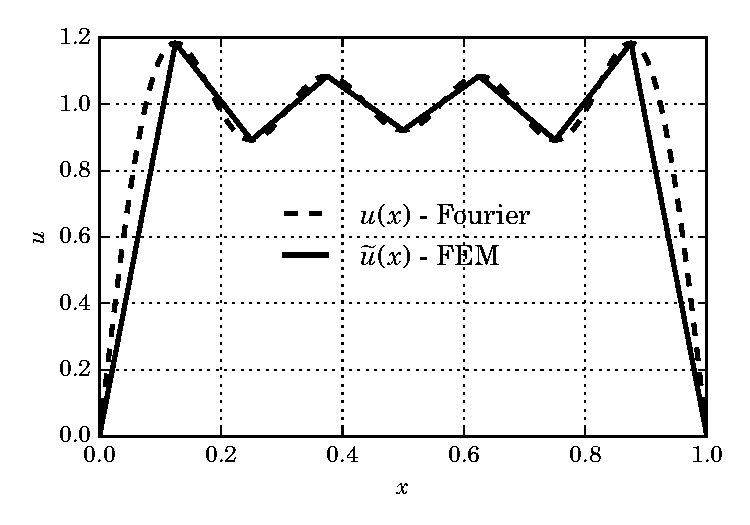
\includegraphics[width=0.7\linewidth]{images/fenics_intro/eigen_solution.pdf}
  \caption[Comparison of FEM with Fourier series solution]{Eight-term Fourier series approximation (dashed) and eight-element finite element approximation (solid) to transient problem \cref{intro_eigen_pde,intro_eigen_bc,intro_eigen_ic} with $\ell = 1$ with $f(x)=1$ at $t=0$.}
  \label{1d_example_eigensolution}
\end{figure*}
